\chapter{Introduction}
% TODO references for these
Cellular Automata (CA) are a very simple model of computation.
There are many variations and extensions of them,
and some like Conway's Game of Life and Rule 110 are known to be Turing Complete.
Isabelle is a proof assistant that can be used for anything from mathematical proofs to formal verification of software properties.


\section{Topic addressed in this project}

This project looks at formalising models of Cellular Automaton in Isabelle to help deal with the complexity that comes with trying to mathematically prove results about them.
In addition to providing a formalisation of six different variants of CA,
this project provides definitions of important properties they may have, and proves some lemmas and theorems necessary to work with them.


\section{Motivation}

It can be very difficult to work with high level concepts while still being rigorous,
and theoretical Computer Science is a very abstract and mathematical discipline that requires exactly that.
One of the main concepts used in theoretical CS is the Turing Machine.
While it provides an excellent way of approaching computation that allows for conceptually easy high level proofs,
being very strict and formal in these can prove difficult.

However the Turing Machine is not the only available model in CS.
One of the goals of this project was to look at \emph{alternative} concepts that achieve the same thing,
to help better appreciate the benefits and drawbacks.
Cellular Automata were chosen as they strike a good balance between simplicity and complexity,
as they have a very simple idea, 
but come with additional geometric aspects to consider.

The motivation to use a proof assistant rather than traditional pen and paper proofs
comes from a desire to use the exactness of computers to cope with issues that stem from highly layered and detailed concepts.


\section{Approach}

\docs{Isabelle} was chosen as the language and framework to implement these models in.
This is due to it being very high level,
and having advanced tools available to ease the creation process.
These include the multitool command \mintinline{isabelle}{sledgehammer} which invokes several Automatic Theorem Provers and Satisfiability-Modulo-Theories solvers, and \mintinline{isabelle}{nitpick} which provides counter-examples to statements.
% TODO put links to docs on sledgehammer/nitpick
These take the burden of large manual proofs off the programmer,
while still encouraging simple and understandable definitions,
as these are more easy to automatically prove results on.

Isabelle also has a powerful and expressive type system,
and the decision was taken to directly make use of this in the CA definitions created.
This involved making each kind of CA explicitly into a type,
to make use of automatic type checking and other benefits.
This contrasts with a more mechanical approach taken in a paper \cite{urban} that also works on implementing Turing Machines and other computability concepts in Isabelle.
One reason for this difference in approach is their work involves the need to convert between different models, for instance Abacus Machine to Turing Machine,
whereas in this project no conversions are done.
Additionally the design of such ``machines'' lend themselves to being built in such a way.
However it was not possible to entirely avoid that way of thinking with CA either, in particular in the two dimensional case.


\section{Metrics}

It can be difficult to evaluate exactly how well a definition has been translated from the informal to the formal.
It could be possible to have a very precise and elegant program that doesn't actually capture the intuitive content of the informal idea.
As such the definitions written here were evaluated in two main ways:

\begin{enumerate}
    \item Understanding: Does reading the program lead to the same understanding as reading the original definitions?
        If so then it is capturing the same spirit as the original,
        even if the means of execution may differ slightly or significantly.
    \item Functionality: As CA are systems that can be run,
        it is necessary to run them on example programs and see the correct results are achieved.
        Speed is not a trait that is sought out but accuracy is of course essential.
\end{enumerate}

Also taken into account is the ability to state properties of these systems,
and the ease or difficulty of proving results about them.



%\begin{figure}[h]
%    \centering
%    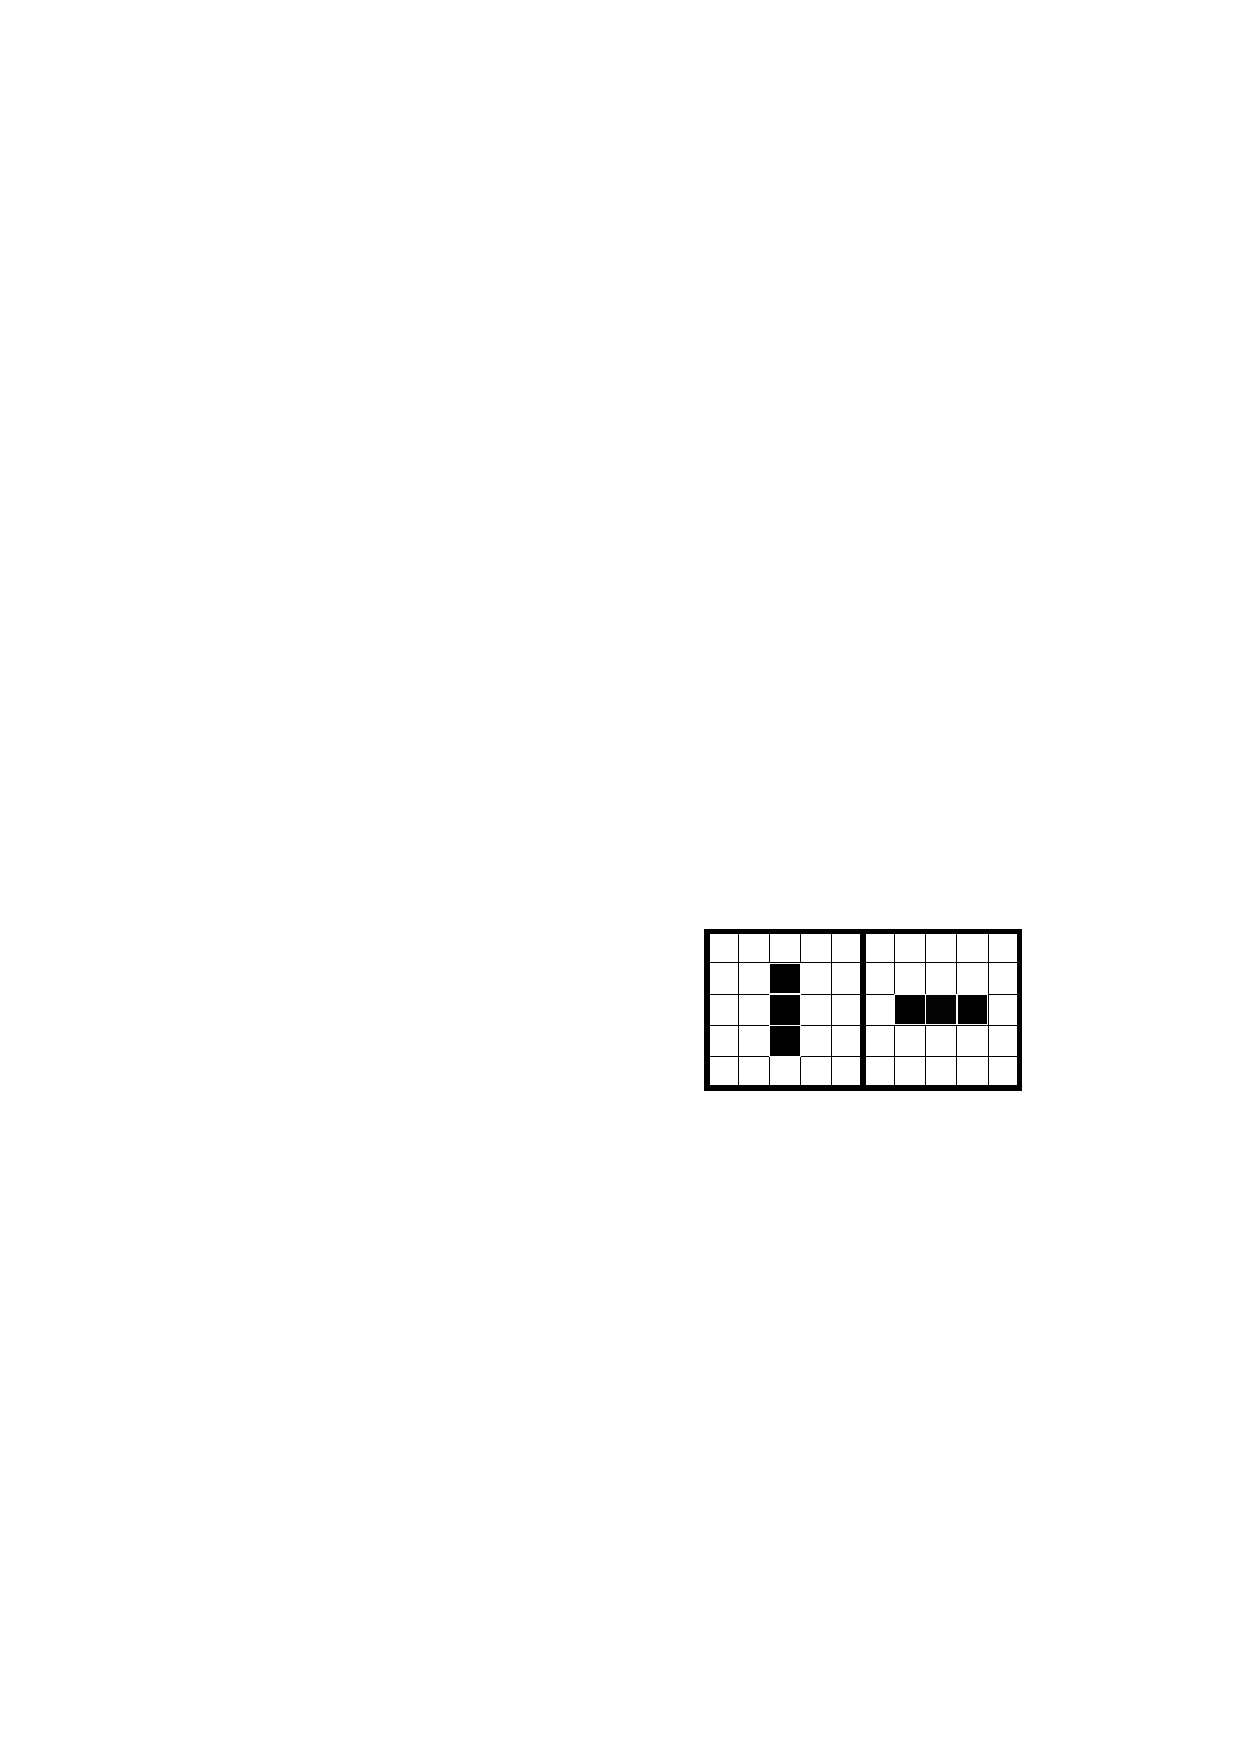
\includegraphics[scale=0.7]{blinkers_both.pdf}
%    \caption{Both forms of a Blinker}
%    \label{fig:binkers}
%\end{figure}

%\begin{myminted}{Some Example Isabelle}{testcode}
%    fun garden_of_eden :: "CA ==> bool" where
%    "garden_of_eden (CA s r) = (¬(EX s0. (CA s0 r) yields s))"
%
%    theorem "ca yields State (run ca 1)"
%    proof-
%      show ?thesis using yields_def by blast
%    qed
%\end{myminted}
